\documentclass[10pt]{article}
\usepackage[sc]{mathpazo}
\usepackage{commands}


\usetikzlibrary{arrows.meta}
\usepackage{cmbright}
\definecolor{green}{rgb}{0.0,0.50,0.0}
\tikzset{>={Straight Barb[angle'=80, scale=1.1]}}

\let\oldphi\phi 
\let\phi\varphi 
\let\varphi\oldphi





\begin{document}

\begin{figure}[h!]
	\centering
	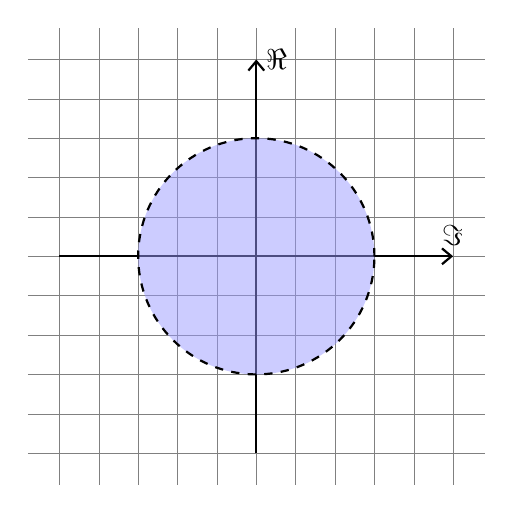
\begin{tikzpicture}
		\draw[step=0.5, black!10!white, help lines](-2.9,-2.9) grid (2.9, 2.9);
		\draw[thick, ->] (-2.5,0) -- (2.5,0) node[anchor=south] {$\Im$};
		\draw[thick, ->] (0,-2.5) -- (0,2.5) node[anchor=west]{$\Re$};
		\filldraw[blue!40!white, thick, dashed, draw=black, fill opacity=0.5] (0,0) circle (1.5cm);
	\end{tikzpicture}
	\caption{The planar set representing $ |z| \le 3 $}
\end{figure}



\begin{figure}[h!]
	\centering
	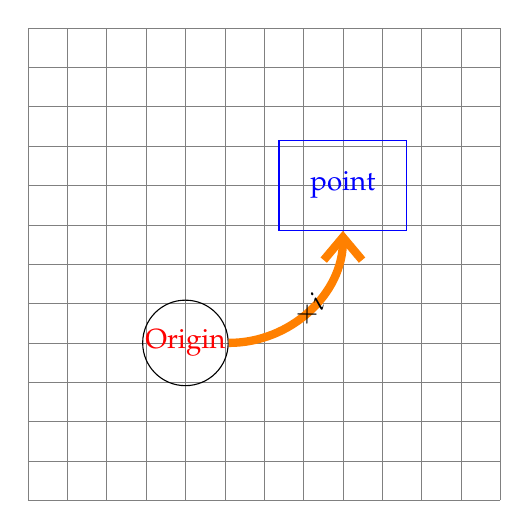
\begin{tikzpicture}[inner sep=4mm]
		\draw [step=0.5, gray, very thin] (-2,-2) grid (4,4);
		\coordinate (O) at (0,0);
		\coordinate (A) at (2,2);
		\node[red, circle, draw=black,inner sep=0.1] (P1) at (O) {Origin};
		\node[blue, rectangle, draw] (P2) at (A) {point};
%		\path (O) node[circle,draw](O) {Origin} (A) node[circle,draw](A) {h};
		\draw[->,orange,line width=3] (P1) to[out=0, in=-90] node[pos=0.5,sloped,black]{$\times i$} (P2);

	\end{tikzpicture}
	\caption{Practicing with nodes}
\end{figure}


\begin{figure}[h!]
	\centering
	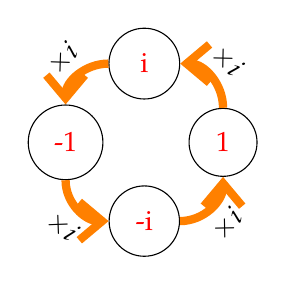
\begin{tikzpicture}[inner sep=4mm]
%		\draw [step=0.5, gray!50!white, line width=0.1] (-2,-2) grid (2,2);
		\node[red, circle, draw=black,inner sep=0.2cm] (1) at (1,0) {1};
		\node[red, circle, draw=black,inner sep=0.23cm] (i) at (0,1) {i};
		\node[red, circle, draw=black,inner sep=0.2cm] (-1) at (-1,0) {-1};
		\node[red, circle, draw=black,inner sep=0.2cm] (-i) at (0,-1) {-i};
		\draw[->, orange, line width=3] (1) to[out=90, in=0] node[sloped, black, anchor=south,inner sep=1mm] {$\times i$} (i);
		\draw[->, orange, line width=3] (i) to[out=-180, in=90] node[sloped, black, anchor=south,inner sep=1mm] {$\times i$} (-1);
		\draw[->, orange, line width=3] (-1) to[out=-90, in=180] node[sloped, black, anchor=north,inner sep=1mm] {$\times i$} (-i);
		\draw[->, orange, line width=3] (-i) to[out=0, in=-90] node[sloped, black, anchor=north,inner sep=1mm] {$\times i$} (1);
	\end{tikzpicture}
	\caption{Practicing with nodes}
\end{figure}




\begin{figure}
	\centering
	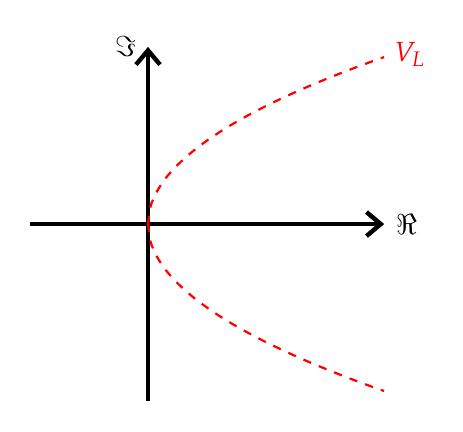
\begin{tikzpicture}[scale=1.5]
		\draw [->, ultra thick] (-1,0) -- (2,0) node [right] {$\Re$};
		\draw [->, ultra thick] (0,-1.5) -- (0,1.5) node [left] {$\Im$};
		\draw[thick,samples=100,smooth,variable=\x,domain=0:2,red, dashed]
		plot(\x,{(\x)^0.5}) node[above=1,right] {$V_L$}
		plot(\x,{-(\x)^0.5});
	\end{tikzpicture}
	\caption{Plotting the functions}
\end{figure}


\begin{figure}
	\centering
	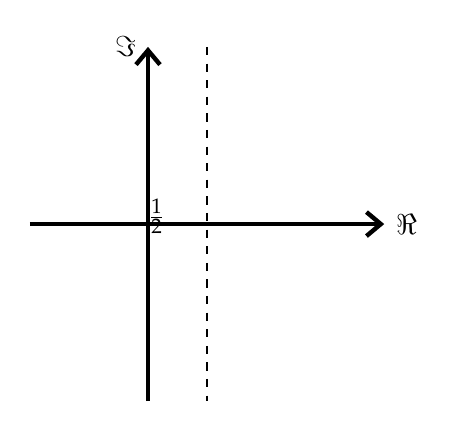
\begin{tikzpicture}[scale=1.5]
		\draw[->, ultra thick] (-1,0) -- (2,0) node [right] {$\Re$};
		\draw[->, ultra thick] (0,-1.5) -- (0,1.5) node [left] {$\Im$};
		\draw[thick, dashed] (0.5,1.5) -- (0.5,-1.5);
		\tick{0.5,0}{90} node[scale=1,below,fill=gray!15] {$\frac{1}{2}$};
	\end{tikzpicture}
	\caption {Sample plot in $\mathbb{C}$}
\end{figure}


\begin{figure}[h!]
	\centering
	\begin{tikzpicture}[scale=2]
		\def\xmax{2.0}
		\def\ymax{1.6}
		\def\R{1.9}
		\def\ang{35}
		\coordinate (O) at (0,0);
		\coordinate (R) at (\ang:\R);
		\coordinate (-R) at (-\ang:\R);
		\coordinate (X) at ({\R*cos(\ang)},0);
		\coordinate (Y) at (0,{\R*sin(\ang)});
		\coordinate (-Y) at (0,{-\R*sin(\ang)});
		\node[fill=mydarkblue,circle,inner sep=0.8] (point) at (R) {};
		
		\node[mydarkblue,above right=-2] at (R) {$z=x+iy=re^{i\phi}$};
		
		\draw[dashed,mydarkblue] (Y) -- (point) -- ++ (0,{0.1-\R*sin(\ang)});
		
		\draw[->,ultra thick] (-0.2*\xmax,0) -- (\xmax+0.05,0) node[right] {Re};
		\draw[->,ultra thick] (0,-\ymax*0.2) -- (0,\ymax+0.05) node[left] {Im};
		\draw[vector] (O) -- (point) node[pos=0.55,above left=-2] {$r$};
		
		\draw pic[->,"$\theta$",mydarkblue,draw=mydarkblue,angle radius=23,angle eccentricity=1.24]
		{angle = X--O--R};
		
		%\tick{X}{90} node[scale=0.9,left=6,below right=-2] {$x = r\cos\theta$};
		\tick{X}{90} node[mydarkblue,scale=1,below=-1] {$x$};
		\tick{Y}{ 0} node[mydarkblue,scale=1,left] {$y$}; %r\sin\theta = 
		
	\end{tikzpicture}
	\caption{A summary of the polar and Cartesian representation of the complex numbers.}
\end{figure}



\begin{figure}
	\centering
	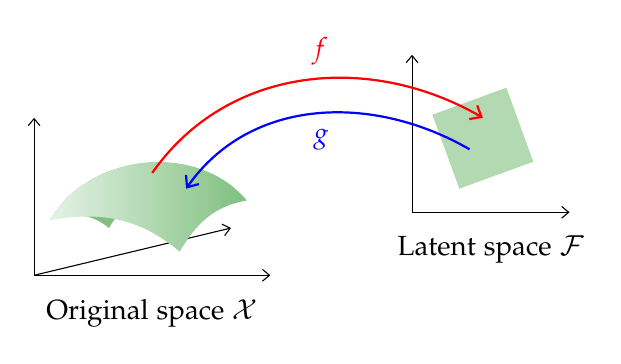
\begin{tikzpicture}
	
		\draw[->] (0, 0) -- ++(0, 2);
		\draw[->] (0, 0) -- ++(2.5, 0.6);
		\draw[->] (0, 0) -- ++(3, 0) node[midway, below, yshift=-0.5em]
		{Original space ${\cal X}$};
		
		\draw[fill=green!50, draw=none, shift={(0.2, 0.7)},scale=0.5]
		(0, 0) to[out=20, in=140] (1.5, -0.2) to [out=60, in=160]
		(5, 0.5) to[out=130, in=60]
		cycle;
		
		\shade[thin, left color=green!10, right color=green!50, draw=none,
		shift={(0.2, 0.7)},scale=0.5]
		(0, 0) to[out=10, in=140] (3.3, -0.8) to [out=60, in=190] (5, 0.5)
		to[out=130, in=60] cycle;
		
		\draw[->] (4.8, 0.8) -- ++(0, 2);
		\draw[->] (4.8, 0.8) -- ++(2, 0) node[midway, below, yshift=-0.5em]
		{Latent space ${\cal F}$};
		
		\draw[thin, fill=green!30, draw=none, shift={(5.4, 1.1)}, rotate=20]
		(0, 0) -- (1, 0) -- (1, 1) -- (0, 1) -- cycle;
		
		\draw[thick,->,red]
		(1.5, 1.3) to [out=55, in=150] node[midway, above, xshift=6pt, yshift=2pt]
		{$f$} (5.7, 2);
		
		\draw[thick,->,blue] (1.5, 1.3) ++(4.03, 0.3) to [out=150, in=55]
		node[midway, below, xshift=2pt, yshift=-2pt] {$g$} ++(-3.6, -0.5);
		
	\end{tikzpicture}

	\caption{Manifold Example}
\end{figure}





\begin{figure}
	\centering
	
	\tikzset{every picture/.style={line width=0.75pt}} %set default line width to 0.75pt        
	
	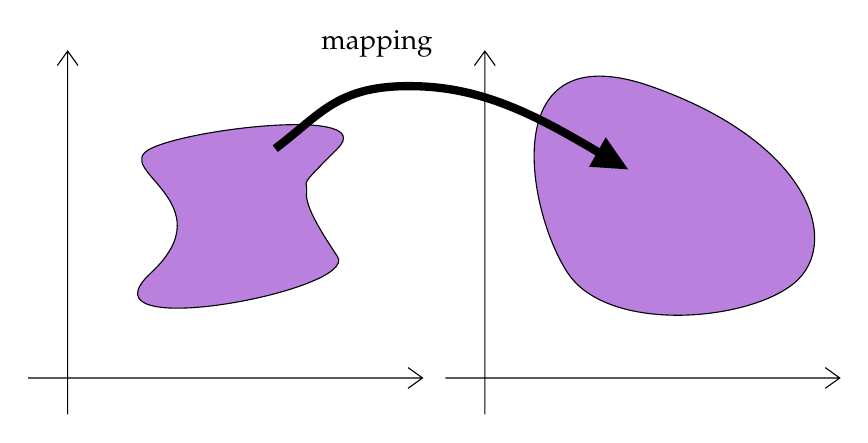
\begin{tikzpicture}[x=0.75pt,y=0.75pt,yscale=-1,xscale=1]
		%uncomment if require: \path (0,300); %set diagram left start at 0, and has height of 300
		
		%Shape: Axis 2D [id:dp5408563926644205] 
		\draw  (81,250.5) -- (271,250.5)(100,93) -- (100,268) (264,245.5) -- (271,250.5) -- (264,255.5) (95,100) -- (100,93) -- (105,100)  ;
		%Shape: Polygon Curved [id:ds6611428337665666] 
		\draw  [fill={rgb, 255:red, 186; green, 255; blue, 221 }  ,fill opacity=1 ] (140,140) .. controls (160,130) and (250,120) .. (230,140) .. controls (210,160) and (215.91,154.51) .. (215.11,160.51) .. controls (214.32,166.51) and (219.13,175.69) .. (230,192) .. controls (240.87,208.31) and (103,234.31) .. (140,200) .. controls (177,165.69) and (120,150) .. (140,140) -- cycle ;
		%Shape: Axis 2D [id:dp043851520245558495] 
		\draw  (282,250.5) -- (472,250.5)(301,93) -- (301,268) (465,245.5) -- (472,250.5) -- (465,255.5) (296,100) -- (301,93) -- (306,100)  ;
		%Shape: Polygon Curved [id:ds5660985402625016] 
		\draw  [fill={rgb, 255:red, 186; green, 255; blue, 221 }  ,fill opacity=1 ] (381,110) .. controls (456,136.31) and (472,183) .. (452,203) .. controls (432,223) and (361,230) .. (341,200) .. controls (321,170) and (306,83.69) .. (381,110) -- cycle ;
		%Curve Lines [id:da23283974936605967] 
		\draw [line width=3]    (200,140) .. controls (222.94,122.8) and (230.37,108.46) .. (270,110) .. controls (307.45,111.46) and (335.99,130.38) .. (364.94,147.11) ;
		\draw [shift={(370,150)}, rotate = 209.47] [fill={rgb, 255:red, 0; green, 0; blue, 0 }  ][line width=0.08]  [draw opacity=0] (16.97,-8.15) -- (0,0) -- (16.97,8.15) -- cycle    ;
		
		% Text Node
		\draw (221,82) node [anchor=north west][inner sep=0.75pt]   [align=left] {mapping};
		
		
	\end{tikzpicture}
	\caption{Mapping}
\end{figure}









\end{document}